%-----------------------------------------------------------------------------%
\chapter{\babDua}
%-----------------------------------------------------------------------------%

%-----------------------------------------------------------------------------%
\section{Ekspresi Gen}
%-----------------------------------------------------------------------------%
Percobaan \textit{microarray}, mengukur tingkat aktivitas gen di dalam sebuah jaringan sel. Sehingga dapat memberikan informasi berdasarkan aktivitas di dalam jaringan yang bersangkutan. Data ini didapatkan dengan cara mengukur banyaknya mRNA yang diproduksi pada saat proses transkripsi DNA, dimana dapat diukur seberapa aktif atau seberapa berfungsinya gen tersebut dalam sebuah jaringan \citep{elloumi2011algorithms}. Karena kanker berhubungan dengan berbagai macam aktivitas penyimpangan regulasi pada sel, maka data ekspresi gen pada kanker merefleksikan penyimpangan regulasi tersebut. Untuk menangkap keabnormalan ini, percbaan microarray, dimana dapat mengukur secara simultan dari level ekspresi ratusan bahkan ribuan ekspresi gen dapat digunakan untuk mengidentifikasi kanker. Percobaan microarray sering dipakai untuk membandingkan profil ekspresi gen pada sel yang terkena kanker, dibandingkan dengan sel yang normal pada berbagai macam percobaan. Percobaan microarray digunakan untuk mengidentifikasi ekspresi yang berbeda pada dua percobaan, yang biasanya berupa data tes dan data kontrol \citep{elloumi2011algorithms}. \\
Ada 23.6\% fungsi gen yang belum diketahui kegunaannya sampai saat ini, hal ini merupakan tantangan pada saat dilakukan proses pengenalan penyakit yang diderita oleh pasien. Dikarenakan ada kemungkinan gen yang sangat berpengaruh terhadap identifikasi penyakit, masih belum diketahui fungsinya. Oleh karena itu, pada proses klasifikasi penyakit dengan menggunakan machine learning, sering digunakan pengenalan secara \textit{unsupervised learning} \citep{haggstrom2014diagram}. \\
\begin{figure}
	\centering
	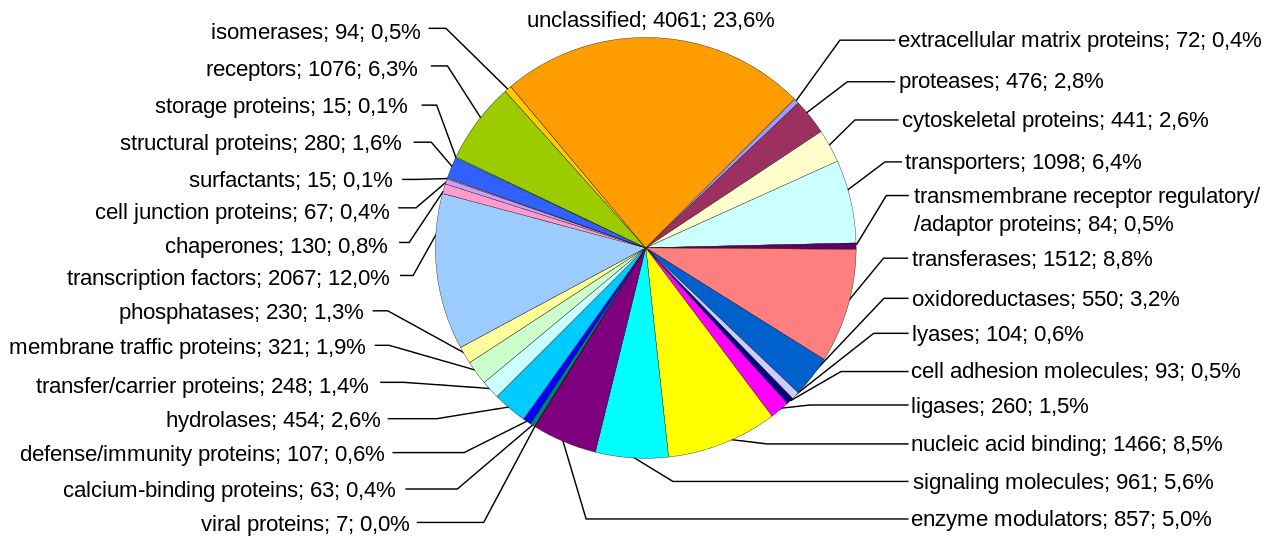
\includegraphics[width=0.50\textwidth]
		{pics/gbr2_1.png}
	\caption{Ada 23,6\% dari keseluruhan fungsi gen yang belum diketahui, sehingga pengetahuan tentang fungsi gen masih belum lengkap. \citep{haggstrom2014diagram}}
	\label{fig:gbr2.1}
\end{figure}

Data ekspresi gen yang masih mentah didapatkan dari percobaan di laboratorium menggunakan alat yang dinamakan dengan alat Genchip microarray. Data tersebut kemudian dilakukan pemrosesan awal untuk mendapatkan sebuah matriks ekspresi gen. Matriks ini memiliki data kolom dan baris, dimana kolom berisi data eksperimen, dan baris berisi nilai ekspresi pada tiap-tiap gen (\pic~\ref{fig:gbr2.2}) \citep{babu2004introduction}.

\begin{figure}
	\centering
	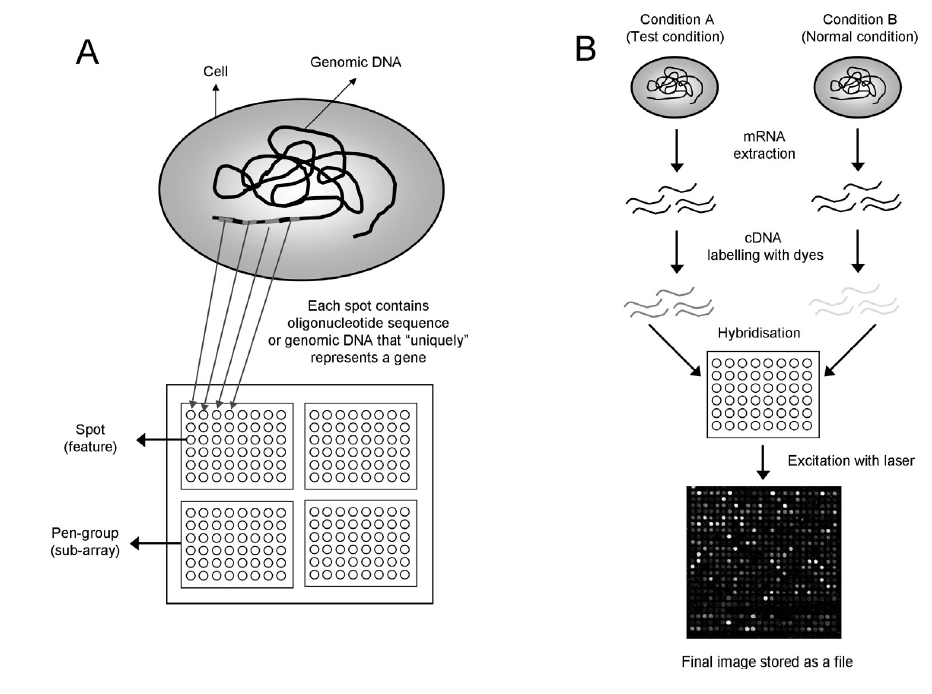
\includegraphics[width=0.95\textwidth]
		{pics/gbr2_2.png}
	\caption{Proses Keseluruhan Percobaan Microarray.\citep{yoon2006building}}
	\label{fig:gbr2.2}
\end{figure}

Pengukuran microarray direspresentasikan dengan tabel gen ekspresi, dimana bagian barisnya adalah fitur ekspresi gen, dan bagian kolom merepresentasikan pasien.

\begin{figure}
	\centering
	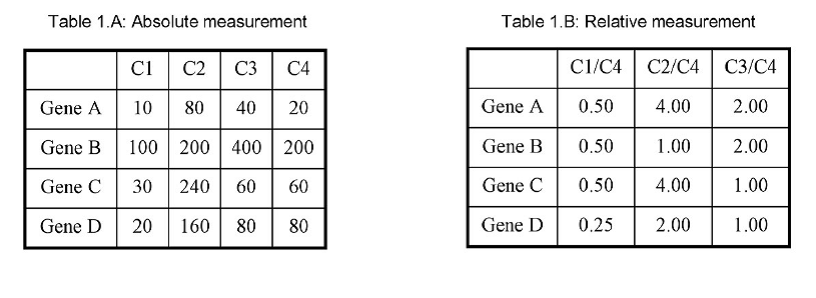
\includegraphics[width=0.95\textwidth]
		{pics/msr.png}
	\caption{Contoh data pengukuran percobaan microarray \citep{yoon2006building}}
	\label{fig:msr}
\end{figure}

Karena data microarray yang didapatkan dapat mencapai ribuan ekspresi dalam satu waktu secara simultan, maka data ini dapat sangat membantu dalam mengidentifikasi penyakit. Akan tetapi, hasil yang didapat dengan menganalisa beberapa data microarray yang dilakukan oleh dua percobaan yang berbeda tetapi dengan tujuan yang sama, dapat menghasilkan hasil yang sangat berbeda. Salah satu alasannya adalah terbatasnya sampel dan terlalu banyaknya profil ekspresi gen. Sehingga diperlukan metode testing statistik untuk memastikan bahwa data microarray tersebut memiliki tingkat signifikansi yang cukup, dan dipastikan bahwa perbedaan tersebut memang karena eksperimen, bukan karena kerusakan alat atau kesalahan prosedur eksperimen.
\begin{figure}
	\centering
	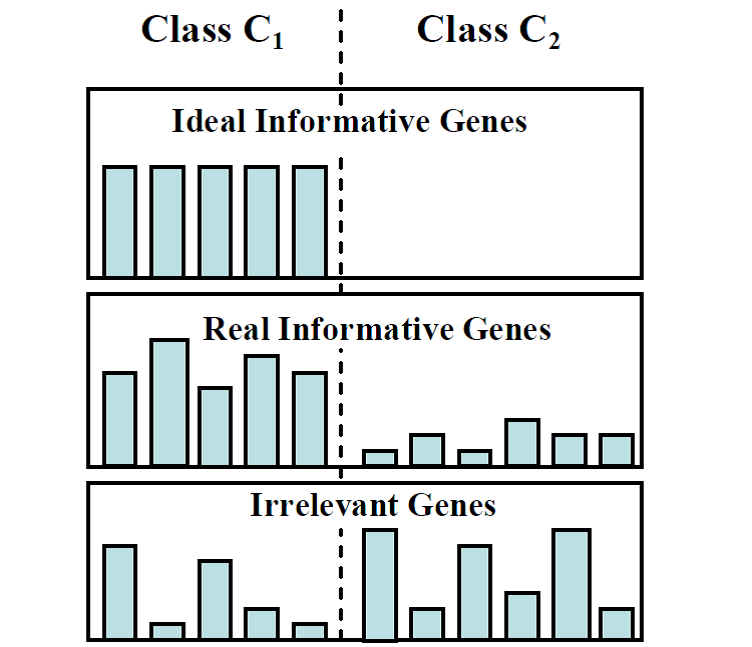
\includegraphics[width=0.8\textwidth]
		{pics/relevansigen.png}
	\caption{Perbandingan Ekspresi gen yang relevan dan informatif dibandingkan dengan gen yang tidak relevan\citep{babu2004introduction}}
	\label{fig:relevansi}
\end{figure}


%-----------------------------------------------------------------------------%
\section{Pemrosesan Data Microarray}
%-----------------------------------------------------------------------------%
Data yang dihasilkan dari alat microarray ini berupa citra yang perlu diproses lebih lanjut. Sebelum data ekspresi gen dapat dianalisa lebih lanjut, perlu dilakukan pemrosesan awal yang berupa (i) perbaikan background, (ii) normalisasi data dan kemudian (iii) penyaringan data.
\begin{enumerate}
\item{\textbf{Perbaikan Background}}\\
Perbiakan background ini ditujukan untuk menghilangkan titik-titik noise yang tidak berasal dari proses hibridisasi. Metode untuk perbaikan background ini banyak diajukan dalam penelitian\citep{fakoorusing}. 
\item{\textbf{Normalisasi}}\\
Tujuan dari normalisasi adalah untuk mengatur bias yang dihasilkan oleh variasi proses percobaan microarray. Metode normalisasi data microarray ada banyak, dan pada penelitian ini akan digunakan normalisasi standar untuk data microarray.
\item{\textbf{Penyaringan data}}
Tidak semua data yang didapat dari percobaan microarray bagus, kadangkala terjadi kesalahan alat dan noise yang diakibatkan oleh alat, oleh karena itu perlu disaring, mana data yang disebabkan oleh proses biologi, dan mana yang disebabkan oleh noise alat.
\item{\textbf{Missing Value Imputation}}\\
Tidak semua data ekspresi gen dapat kita dapatkan, dikarenakan rumitnya percobaan microarray, kadangkala data tidak kita dapatkan, oleh sebab itu diperlukan metode untuk melakukan pendekatan statistic dalam memberikan perkiraan isi data dalam titik data yang hilang tersebut.
\item{\textbf{Seleksi Fitur}}\\
Setelah proses diatas, diperlukan teknik untuk menseleksi fitur pada data microarray. Ada banyak metode yang sudah diusulkan oleh para peneliti. Seperti pada table 1 dibawah. Dan pada titik inilah penelitian ini dijalankan. Diharapkan penelitian ini menghasilkan metode reduksi dimensi untuk data microarray.

\end{enumerate}

%-----------------------------------------------------------------------------%
\section{Ekstraksi Fitur dan Seleksi Fitur Pada Penelitian Sebelumnya}
%-----------------------------------------------------------------------------%
Pada tabel dibawah ditunjukkan perbandingan penelitian-penelitian ekstraksi fitur dengan menggunakan berbagai macam metode.
% Please add the following required packages to your document preamble:
% \usepackage{booktabs}
% \usepackage[normalem]{ulem}
% \useunder{\uline}{\ul}{}
\begin{table}
\centering
\caption{Perbandingan Metode Seleksi fitur  pada dataset microarray}
\label{my-label}
\begin{tabular}{@{}llll@{}}
\toprule
Pengarang                                                            & Judul Paper                                                                                                                                                                     & Metode                                                                                                                            & Dataset                                                           \\ \midrule
\begin{tabular}[c]{@{}l@{}}C. Aliferis et al. \\ 2003\end{tabular}   & \begin{tabular}[c]{@{}l@{}}Machine learning models \\ for classication  of lung \\ cancer and selection of \\ genomic markers using \\ array gene expression data.\end{tabular} & \begin{tabular}[c]{@{}l@{}}Reduksi fitur secara rekursif \\ dan melakukan filter secara \\ asosiasi univariate\end{tabular}       & \begin{tabular}[c]{@{}l@{}}Lung Cancer \\ Microarray\end{tabular} \\
\begin{tabular}[c]{@{}l@{}}Ramaswamy, S. \\ et al. 2001\end{tabular} & \begin{tabular}[c]{@{}l@{}}Multiclass cancer diagnosis \\ using tumor gene expression \\ signatures.\end{tabular}                                                               & \begin{tabular}[c]{@{}l@{}}Pengurangan fitur secara \\ rekursif dengan \\ mengguanakan SVM\end{tabular}                           & \begin{tabular}[c]{@{}l@{}}Various \\ Microarray\end{tabular}     \\
\begin{tabular}[c]{@{}l@{}}Wang et al., \\ 2005\end{tabular}         & \begin{tabular}[c]{@{}l@{}}Gene-expression proles to \\ predict distant  metastasis \\ of lymph-node-negative \\ primary breast cancer.\end{tabular}                            & \begin{tabular}[c]{@{}l@{}}Mengkombinasikan seleksi \\ fitur yang  berbasis korelasi \\ dengan pendekatan assosiasi.\end{tabular} & \begin{tabular}[c]{@{}l@{}}Various \\ Microarray\end{tabular}     \\
\begin{tabular}[c]{@{}l@{}}Sharma et. Al, \\ 2012\end{tabular}       & \begin{tabular}[c]{@{}l@{}}Combining multiple \\ approaches for gene \\ microarray classification.\end{tabular}                                                                 & \begin{tabular}[c]{@{}l@{}}Mengkombinasikan banyak\\   pendekatan ekstraksi fitur\end{tabular}                                    & \begin{tabular}[c]{@{}l@{}}Various \\ Microarray\end{tabular}     \\ \bottomrule
\end{tabular}
\end{table}


%-----------------------------------------------------------------------------%
\section{Deep Learning}
%-----------------------------------------------------------------------------%

Sebelum tahun 2006, melakukan training dalam arsitektur \textit{deep learning} selalu gagal. Percobaan untuk melakukan training dengan \textit{feedforward neural network} memiliki hasil yang lebih buruk dibandingkan dengan arsitektur yang dangkal, yaitu arsitektur dengan layer 1 atau maksimum 2 layer.\\
Akan tetapi tiga paper yang terbit pada 2006 secara revolusioner telah merubah hal terssebut. Sehingga setelah tahun 2006 penelitian tentang \textit{deep learning} menjadi lebih intensif sampai sekarang dengan segala variasi arsitekturnya. Salah satu variasi arsitektur \textit{deep learning} yang dipakai dalam thesis ini adalah \textit{arsitektur Deep Believe Network (DBN)}. Ketiga paper tersebut adalah:
\begin{enumerate}
\item Hinton, G. E., Osindero, S. and Teh, Y., A fast learning algorithm for deep belief nets Neural Computation 18:1527-1554, 2006 \citep{hinton2006fast}
\item Yoshua Bengio, Pascal Lamblin, Dan Popovici and Hugo Larochelle, Greedy Layer-Wise Training of Deep Networks, in J. Platt et al. (Eds), Advances in Neural Information Processing Systems 19 (NIPS 2006), pp. 153-160, MIT Press, 2007 \citep{bengio2007greedy}.
\item Marc’Aurelio Ranzato, Christopher Poultney, Sumit Chopra and Yann LeCun Efficient Learning of Sparse Representations with an Energy-Based Model, in J. Platt et al. (Eds), Advances in Neural Information Processing Systems (NIPS 2006), MIT Press, 2007\citep{poultney2006efficient}.
\end{enumerate}


Learning secara \textit{unsupervised} menggunakan \textit{pretraining} secara tiap layer yang disebut dengan \textit{greedy layer-wise training}, yaitu training dilakukan  satu layer pada tiap satu waktu. Training ini dilakukan secara berjenjang pada layer selanjutnya. Kemudian dilakukan \textit{supervised training} untuk melakukan \textit{tuning parameter}, yang dimulai dari parameter hasil pretraining yang dilakukan sebelumnya.\\
DBN menggunakan RBM sebagai bagian terkecil dari layernya, yang menggunakan learning secara unsupervised yang merepresentasikan tiap layer. Sejak 2006, banyak sekali paper-paper yang mulai melakukan eksplorasi tentang deep learning ini, sehingga sejak saat itu deep learning merupakan salah satu teknik \textit{machine learning} yang paling populer, bahkan sampai saat ini \citep{fakoorusing}.

\section{Energy-Based Model (EBM)}

EBM mengaitkan sebuah energi skalar pada setiap konfigurasi variable yang diinginkan. Proses learning bertujuan untuk memodifikasi fungsi energi sehingga bentuknya memiliki  sifat yang diinginkan. Sebagai contoh, misalnya diinginkan sebuah bentuk konfigurasi yang memiliki energi yang rendah, maka model probabilistik dari EBM didifinisikan sebagi distribusi probabilitas melalui fungsi energi sebagi berikut\citep{poultney2006efficient}
\begin{equation}
p(x) = \frac {e^{-E(x)}} {Z}.
\end{equation}

Z adalah faktor normalisasi yang disebut sebagai fungsi partisi untuk menganalogikan dengan sistem fisika.
\begin{equation}
Z = \sum_x e^{-E(x)}
\end{equation}


EBM bisa dilatih dengan cara melakukan (stochastic) gradient descent pada negative log-likelihood (NLL)-nya secara empiris pada data training. Adapun untuk logistic regression akan didifinisikan terlebih dahulu log-likelihood $\mathcal{L}(\theta, \mathcal{D})$ dan fungsi loss-nya sebagai NLL $\ell (\theta, \mathcal{D})$ sebagai berikut:
\begin{equation}
\begin{aligned}
\mathcal{L}(\theta, \mathcal{D}) &= \frac{1}{N} \sum_{x^{(i)} \in
\mathcal{D}} \log\ p(x^{(i)}) \\
\ell (\theta, \mathcal{D}) &= - \mathcal{L} (\theta, \mathcal{D})
\end{aligned}
\end{equation}


Menggunakan stochastic gradient $-\frac{\partial  \log p(x^{(i)})}{\partial
\theta}$, dimana $\theta$ adalah parameter dari modelnya\citep{poultney2006efficient}.

\subsection{EBM dengan Hidden Units}

Pada banyak kasus, sampel $x$ biasanya tidak terobservasi secara penuh, atau akan ditambahkan variabel yang tidak terobservasi secara langsung yang disebut dengan hidden unit, dimana hal ini berguna untuk meningkatkan ekspresivitas dari model. Sehingga dikenalkan bagian yang terobservasi disini dilambangkan dengan $x$, dan sebuah bagian yang tersembunyi dilambangkan dengan $h$. Sehingga bisa ditulis sebagai:
\begin{equation}
P(x) = \sum_h P(x,h) = \sum_h \frac{e^{-E(x,h)}}{Z}.
\end{equation}

Pada kasus ini, untuk melakukan pemetaan rumus yang mirip dengan rumus 2.4 , akan dikenalkan notasi (yang merupakan inspirasi dari fisika) yaitu free energy $\mathcal{F}(x)$, yang didifinisikan sebagai berikut:

\begin{equation}
\mathcal{F}(x) = - \log \sum_h e^{-E(x,h)}
\end{equation}

Sehingga bisa diturunkan sebagai :
\[P(x) = \frac{e^{-\mathcal{F}(x)}}{Z} \text{ dengan } Z=\sum_x e^{-\mathcal{F}(x)}.\]

Data dari gradien NLL kemudian memiliki bentuk yang menarik yaitu:
\begin{equation}
- \frac{\partial  \log p(x)}{\partial \theta}
 = \frac{\partial \mathcal{F}(x)}{\partial \theta} -
       \sum_{\tilde{x}} p(\tilde{x}) \
           \frac{\partial \mathcal{F}(\tilde{x})}{\partial \theta}.
\end{equation}

Gradien diatas memiliki dua istilah, dimana hal tersebut mereferensikan pada fase positif dan fase negatif. Istilah positif dan negatif ini tidak merujuk pada tanda (positif/negatif)  persamaan, akan tetapi merefleksikan efek pada kepadatan probabilitas yang didefinisikan oleh model. Istilah pertama, menambah probabilitas data training (dengan cara mengurangi free energy yg berhubungan), sedangkan istilah kedua mengurangi probabilitias sampel yang digenerasi oleh model \citep{poultney2006efficient}.\\

Biasanya sulit untuk menentukan gradien secara analitis, oleh karena berhubungan dengan komputasi dari $E_P [ \frac{\partial \mathcal{F}(x)} {\partial \theta} ]$. Dikarenakan hal ini merupakan ekspektasi semua kemungkinan konfigurasi input $x$ (pada distribusi $P$ yang dibentuk oleh model).\\
Oleh karena itu, langkah pertama agar bisa dikomputasi secara analitis maka dilakukan estimasi ekspektasi menggunakan jumlah yang pasti dari sampel pada model. Sampel digunakan untuk mengestimasi gradien dari fase negatif yang direferensikan sebagai partikel negatif, dimana disimbolkan sebagai $\mathcal{N}$. Kemudian, gradien bisa ditulis sebagai \citep{poultney2006efficient} : 

\begin{equation}
- \frac{\partial \log p(x)}{\partial \theta}
 \approx
  \frac{\partial \mathcal{F}(x)}{\partial \theta} -
   \frac{1}{|\mathcal{N}|}\sum_{\tilde{x} \in \mathcal{N}} \
   \frac{\partial \mathcal{F}(\tilde{x})}{\partial \theta}.
\end{equation}
Dimana secara ideal, elemen seperti $\tilde{x}$ dari $\mathcal{N}$ disampel menurut $P$ (sebagai contoh adalah menggunakan teknik sampling Monte-Carlo). Dengan rumus diatas, secara praktis hampir bisa melakukan algoritma stochastic, hanya saja partikel negatif $\mathcal{N}$ belum bisa diekstraksi. Oleh karena itu, pada literatur dengan metode Markov Chain Monte Carlo, sangat bagus digunakan pada model Restricted Boltzmann Machine (RBM) yang merupakan bentuk spesifik dari model EBM \citep{tutorial2014lisa}.


%-----------------------------------------------------------------------------%
\section{Restricted Boltzmann Machine}
%-----------------------------------------------------------------------------%
Boltzmann Machines (BMs) adalah bentuk khusus dari log-linear Markov Random Field (MRF), dengan kata lain, dimana fungsi energi adalah linear pada parameter bebasnya. Agar membuat BM cukup bisa merepresentasikan distribusi yang kompleks(dengan kata lain, berangkat dari setting parameter yang terbatas kepada non paramter), diasumsikan bahwa beberapa variabel tidak terobserbasi sehingga disebut hidden. Dengan memiliki variabel hidden, bisa dilakukan peningkatan kapasitas model dari BM. RBM, selanjutnya membuat BM yang terbatas pada variabel tanpa koneksi visibel-visibel dan hidden-hidden. Seperti pada gambar \ref{fig:rbm} \citep{hinton2006fast}\\
\begin{figure}
	\centering
	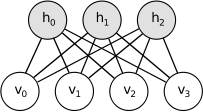
\includegraphics[width=0.3\textwidth]
		{pics/rbm.png}
	\caption{Grafik yang Menggambarkan RBM}
	\label{fig:rbm}
\end{figure}

Fungsi energi $E(v,h)$ pada RBM didefinisikan sebagai persamaan \ref{eq:rbm1}.

\begin{equation}
E(v,h) = - b'v - c'h - h'Wv
\label{eq:rbm1}
\end{equation}

Dimana $W$ merepresentasikan bobot yang terkoneksi antara unit hidden dan visible dan $b$, $c$ adalah bias dari visible dan hidden secara berurutan.\\

Hal ini bisa diterjemahkan dalam bentuk persamaan energi bebas $\mathcal{F}(v)$ seperti dibawah:
\[\mathcal{F}(v)= - b'v - \sum_i \log \sum_{h_i} e^{h_i (c_i + W_i v)}.\]
Dikarenakan struktur RBM yang spesifik, visibel dan hidden adalah independen secara bersyarat antara satu dengan lainnya. Dengan menggunakan sifat tersebut, maka dapat dituliskan :

\[p(h|v) = \prod_i p(h_i|v)\]
\[p(v|h) = \prod_j p(v_j|h).\]

\subsection{RBMs yang Menggunakan Unit Biner}

Kasus umum jika menggunakan unit biner (dimana $v_j$ dan $h_i \in
\{0,1\})$, yang didapat dari persamaan (6) dan (2), versi probabilistik dari fungsi aktivasi neuron adalah sebagai berikut\citep{hinton2006reducing}:

\begin{equation}
P(h_i=1|v) = sigm(c_i + W_i v)
\end{equation}

\begin{equation}
P(v_j=1|h) = sigm(b_j + W'_j h)
\end{equation}

Selanjutnya, energi bebas dari RBM dengan unit biner, disederhanakan menjadi persamaan:

\begin{equation}
\mathcal{F}(v)= - b'v - \sum_i \log(1 + e^{(c_i + W_i v)}).
\end{equation}

\subsection{Update Persamaan dengan Unit Biner}

Menghubungkan persamaan (5) dengan (9), didapatkan gradien log-likelihood untuk RBM dengan unit biner sebagai berikut:

\begin{equation}
\begin{aligned}
- \frac{\partial{ \log p(v)}}{\partial W_{ij}} &=
    E_v[p(h_i|v) \cdot v_j]
    - v^{(i)}_j \cdot sigm(W_i \cdot v^{(i)} + c_i) \\
-\frac{\partial{ \log p(v)}}{\partial c_i} &=
    E_v[p(h_i|v)] - sigm(W_i \cdot v^{(i)})\\
-\frac{\partial{ \log p(v)}}{\partial b_j} &=
    E_v[p(v_j|h)] - v^{(i)}_j
\end{aligned}
\label{eq:eq2.10}
\end{equation}

\section{Sampling pada RBM}

Sampel dari $p(x)$ bisa didapat dengan menjalankan Markov chain sampai konvergen dengan menggunakan gibbs samping sebagai operator transisi. \\

Gibbs sampling dari join variable random sebanyak $N$ dari $S=(S_1, ... , S_N)$ merupakan urutan sebanyak $N$ sampling dari sub-steps dalam bentuk $S_i \sim p(S_i | S_{-i})$ dimana $S_{-i}$ berisi $N-1$ variabel random lain didalam $S$ tetapi diluar $S_i$.

Untuk RBM, $S$ berisi himpunan dari visible dan hidden unitnya. Akan tetapi, dikarenakan unit ini dipenden secara kondisional, maka salah satunya bisa dilakukan gibbs sampling. Pada setting disini, unit visible disampel secara simultan given nilai fix dari hidden unitnya. Demikian sebaliknya, hidden unitnya disampel secara simultan given unit visibelnya.Sehingga satu langkah Markov chain adalah sebagai berikut: 

\[h^{(n+1)} \sim sigm(W'v^{(n)} + c)\] 
\[v^{(n+1)} \sim sigm(W h^{(n+1)} + b),\]

Dimana $h^{(n)}$ menunjik pada himpunan semua hidden unit pada nilai yang ke-$n$ langkah dari Markov chain. Yang artinya adalah sebagai contoh, $h^{(n+1)}_i$ adalah secara random dipilih antara 1 (versus 0) dengan nilai probabilitas $sigm(W_i'v^{(n)} + c_i)$, demikian juga, $v^{(n+1)}_j$ adalah dipilih secara random antara 1 (versus 0) dengan probabilitas $sigm(W_{.j} h^{(n+1)} + b_j)$.

Hal ini seperti digambarkan pada gambar \ref{fig:markov_chain}
\begin{figure}
	\centering
	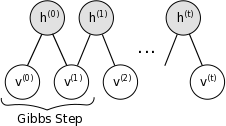
\includegraphics[width=0.3\textwidth]
		{pics/markov_chain.png}
	\caption{Gibbs Sampling}
	\label{fig:markov_chain}
\end{figure}


Oleh karena $t \rightarrow \infty$, maka sampel $(v^{(t)}, h^{(t)})$ bisa dipastikan akan akurat dalam mensampel $p(v,h)$.

Secara teori, tiap parameter diupdate pada proses learning dibutuhkan satu rantai tersebut untuk konvergen. Akan tetapi hal ini sangat mahal komputasinya. Sehingga banyak diajukan algoritma untuk melatih RBM agar sampel $p(v,h)$ efisien, disaat proses learningnya.

\section{Contrastive Divergence (CD-k)}

Contrastive Divergence(CD) menggunakan trik untuk mempercepat proses sampling: Dikarenakan yang diinginkan adalah $p(v) \approx p_{train}(v)$ (distribusi data yang asli), initialisasi  Markov chain dengan contoh data training (dimana, berasal dari distribusi yang mendekati $p$, pada distribusi final dari $p$). CD tidak menunggu rantai untuk konvergen. Sampel didapatkan setalah langkah ke-$k$ dari Gibbs sampling. Pada prakteknya, $k=1$ sudah menghasilkan hasil yang baik.\\

\section{Persistent CD}

Persistent CD (P-CD) [Tieleman08] menggunakan pendekatan lain untuk mensampling $p(v,h)$. Hal ini bergantung hanya pada Markov chain tunggal, yang memiliki kondisi yang persisten (dimana, tidak melakukan restart chain pada setiap sampel yang terobservasi). Pada setiap umpdate parameter, akan di ekstraksi sampel baru dengan penjalankan chain pada langkah ke-$k$. Kondisi chain akan dipertahankan pada update selanjutnya.\\
Intuisinya adalah jika update parameternya cukup kecil dibaningkan dengan rate campuran dari Markov Chain, maka hal ini bisa mengejar perubahan modelnya.



%-----------------------------------------------------------------------------%
\section{Deep Believe Network}
%-----------------------------------------------------------------------------%

\cite{hinton2006fast} menunjukkan bahwa RBM bisa dijajar dan dilatih secara greedy untuk membentuk sebuah jaringan yang dinamakan dengan \textit{Deep Belief Network (DBN)}. DBN adalah model grafis dimana bisa melakukan learning untuk mengekstraksi representasi hirarki yang mendalam (deep) dari data training. Hal ini memodelkan distribusi gabungan antara vektor $x$ sebagai observer dan $\ell$ layer hidden $h^k$ sebagai berikut:

\begin{equation}
P(x, h^1, \ldots, h^{\ell}) = \left(\prod_{k=0}^{\ell-2} P(h^k|h^{k+1})\right) P(h^{\ell-1},h^{\ell})
\end{equation}

Dimana $x=h^0, P(h^{k-1} | h^k)$ adalah distribusi kondisional untuk unit visible dikondisikan pada unit hidden pada level $k$ dan  $P(h^{\ell-1}, h^{\ell})$ adalah distribusi gabungan visible-hidden pada level teratas dar RBM. Seperti diilustrasikan pada gambar \ref{fig:dbn3}.

\begin{figure}
	\centering
	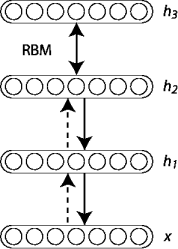
\includegraphics[width=0.3\textwidth]
		{pics/DBN3.png}
	\caption{Arsitektur Deep Believe Network (DBN) yang merupakan gabungan dari RBM yang dibuat bertingkat}
	\label{fig:dbn3}
\end{figure}


Prinsip dari \textit{greedy layer-wise unsupervised training} bisa di aplikasikan pada DBN dengan RBM sebagai bagian pada tiap layernya [hinton] [bengio]. Pada prinsipnya prosesnya adalah sebagai berikut:
\begin{enumerate}
\item Latih layer pertama ssebagai RBM yang memodelkan input $x = h^{(0)}$ sebagai visible layernya.
\item Gunakan layer pertama untuk mendapatkan representasi input yang digunakan sebagai data untuk layer kedua. Ada dua solusi yang sama. Representasi ini bisa dipilih sebagai rata-rata dari aktivasi $p(h^{(1)}=1|h^{(0)})$ atau sampel dari $p(h^{(1)}|h^{(0)})$.
\item Train layer kedua sebagai RBM dengan mengambil data transformasi (sampel atau rata-rata aktivasi) sebagai training (untuk layer visible dari RBM tersebut).
\item Iterasikan (2 dan 3) untuk semua layer yang diinginkan, setiap waktu dengan mempropagasikan keatas antara sampel atau nilai rata-ratanya.
\item Fine-tune semua parameter dari arsitektur dengan log-likelihood DBN atau dengan kriteria secara supervised setelah menambahkan layer supervised untuk memprediksikan kelas, sebagai contoh misalnya layer logistic regression.
\end{enumerate}

Pada kasus ini, akan difokuskan pada fine-tuning dengan melakukan gradien descent menggunakan klassifier logistic regression dimana digunakan untuk mengklasifikasikan input x berdasar pada output dari hidden layer $h^{(l)}$ dari DBN. Fine-tune kemudian dilakukan melalui gradien descent dari NLL fungsi costnya. Dikarenakan gradien secara supervised adalah hanya non-null untuk bobot dan bias pada hidden layer pada tiap-tiap layer, maka prosedur ini serupa dengan menerapkan initialisasi parameter dari arsitektur MLP yang deep dengan bobot dan bias dari hidden layer yang didapat pada proses training unsupervised diatas.


\section{Alasan Melakukan Training Secara Greedy Layer-Wise}

Algoritma training deep learning secara greedy layer-wise terbukti bisa bekerja dengan baik, sebagai contoh 2 layer DBN dengan hidden layer $h^{(1)}$ dan $h^{(2)}$ dengan parameter bobot berurutan adalah $W^{(1)}$ dan $W^{(2)}$, \citep{hinton2006reducing} maka $\log
p(x)$ bisa ditulis sebagai:
\begin{equation}
\begin{aligned}
\log p(x) = &KL(Q(h^{(1)}|x)||p(h^{(1)}|x)) + H_{Q(h^{(1)}|x)} + \\
            &\sum_h Q(h^{(1)}|x)(\log p(h^{(1)}) + \log p(x|h^{(1)})).
\end{aligned}
\label{eq:equ2}
\end{equation}

$KL(Q(h^{(1)}|x) || p(h^{(1)}|x))$ merepresentasikan KL divergence antara posterior $Q(h^{(1)}|x)$ dari RBM pertama jika hal ini sendirian, dan probabilitas $p(h^{(1)}|x)$ untuk layer sayng sama tapi didifinisikan oleh keseluruhan DBN (sebagai contoh, perhitungan prior $p(h^{(1)},h^{(2)}$) didefinisikan sebagai top-level RBM). $H_{Q(h^{(1)}|x)}$ adalah entropy dari distribusi $Q(h^{(1)}|x)$.\\
Hal ini bisa ditunjukkan bahwa jika diinitialisasi kedua layer hidden sehingga $W^{(2)}={W^{(1)}}^T, Q(h^{(1)}|x)=p(h^{(1)}|x)$ dan KL divergence nya adalah null. Maka jika di lakukan learning pada level awal RBM dan kemudian parameter $ W^{(1)}$ dibuat tetap, kemudian dilakukan optimasi pada persamaan \ref{eq:equ2} terhadap $W^{(2)}$ bisa meningkatkan likelihood dari $p(x)$.
Jika diisolasi hanya pada $W^{(2)}$ sehinggi didapatkan:

\[\sum_h Q(h^{(1)}|x)p(h^{(1)})\]

Melakukan optimasi persamaan ini dengan memperhatikan jumlah $W^{(2)}$ training pada tingkat RBM selanjutnya, menggunakan output dari $Q(h^{(1)}|x)$ sebagai distribusi training untuk RBM yang pertama.

%-----------------------------------------------------------------------------%
\section{Logistic Regression}
%-----------------------------------------------------------------------------%
\textit{Logistic Regression} adalah salah satu klassifier yang paling dasar pembentuk dari MLP. Penjelasannya akan dimulai dari bentuk model dasarnya serta notasi matematisnya.

\subsection{Model Logistic Regression}
\textit{Logistic regression} adalah klasifier yang linear dan probabilistik. Diparameterkan dengan matrik bobot $W$ dan vektor bias $b$. Proses klasifikasinya adalah dengan cara memproyeksikan vektor input kedalam himpunan \textit{hyperplane}, dimana berkorespondensi pada kelasnya. Jarak dari input ke \textit{hyperplane} merefleksikan probabilatas dari input adalah berkorespondensi dari anggota kelasnya.\\
Secara matematis, probabilitas vektor input $x$ adalah anggota dari kelas $i$, isi dari variabel \textit{stochastic} $Y$, bisa ditulis sebagai berikut:
\begin{equation}
\begin{aligned}
P(Y=i|x, W,b) &= softmax_i(W x + b) \\
              &= \frac {e^{W_i x + b_i}} {\sum_j e^{W_j x + b_j}}
\end{aligned}
\end{equation}

Prediksi dari model berupa $y_{pred}$ adalah kelas dimana probabilitasnya maksimal, secara spesifik ditulis sebagai:
\begin{equation}
y_{pred} = {\rm argmax}_i P(Y=i|x,W,b)
\end{equation}

\subsection{Mendefinisikan Lost Function dari Logistic Regression}
Melakukang \textit{learning} pamameter model dengan cara meminimalisasi \textit{Lost Function}. Pada kasus \textit{logistic regression} yang multi-kelas, sangat umum digunakan minimisasi \textit{negative log likelihood (NLL)} yang ekivalen dengan memaksimalkan likelihood dari data set $\cal{D}$ pada model yang diparameterkan oleh $\theta$. Definisi dari likelihood $\cal{L}$ dan loss $\ell$ maka:
\begin{equation}
\begin{aligned}
\mathcal{L} (\theta=\{W,b\}, \mathcal{D}) =
  \sum_{i=0}^{|\mathcal{D}|} \log(P(Y=y^{(i)}|x^{(i)}, W,b)) \\
\ell (\theta=\{W,b\}, \mathcal{D}) = - \mathcal{L} (\theta=\{W,b\}, \mathcal{D})
\end{aligned}
\end{equation}
Untuk meminimisasi, digunakan \textit{stochastic gradient descen with minibatches (MSGD)} \citep{hinton2006fast}.


%-----------------------------------------------------------------------------%
\section{Multi Layer Perceptron}
%-----------------------------------------------------------------------------%

Arsitektur selanjutnya yang akan dibahas adalah \textit{Multi Layer Perceptron (MLP)} Arsitektur MLP ini bisa dilihat sebagai klasifier \textit{Logistic Regression} dimana input pada awalnya ditransformasikan menggunakan transformasi non linear $\Phi$. Transformasi ini memproyeksikan data input kepada \textit{space} dimana hal ini bisa terseparasi secara linear. Layer tengah ini direferensikan sebagai \textit{hidden layer}. Satu hidden layer sebenarnya sudah cukup untuk membuat MLP sebagai aproksimator universal. Akan tetapi, ada banyak keuntungan untuk menggunakan hidden unit yang lebih dari satu layer, hal inilah yang digunakan sebagai konsep dasar dari deep learning. Algoritma untuk melakukan \textit{training} dari MLP yang paling sering dipakai adalah algoritma \textit{back-propagation} \citep{tutorial2014lisa}.

\subsection{Model MLP}

MLP atau sering disebut juga dengan Artificial Neural Network (ANN) adalah Perceptron yang dibentuk menjadi sebuah jaringan. MLP dengan layer tunggal bisa direpresentasikan secara grafis seperti pada  \pic~\ref{fig:mlp} berikut.

\begin{figure}
	\centering
	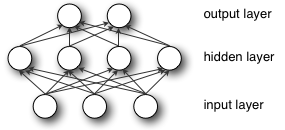
\includegraphics[width=0.45\textwidth]
		{pics/mlp.png}
	\caption{Arsitektur Layer Tunggal MLP}
	\label{fig:mlp}
\end{figure}

Secara formal, hidden layer tunggal dari MLP adalah sebuah fungsi $f: R^D \rightarrow R^L$, dimana $D$ aadlah ukuran dari vektor input $x$ dan $L$ adalah ukuran dari output vektor $f(x)$ sehingga dengan menggunakan notasi matriks sebagai berikut :

\begin{equation}
f(x) = G( b^{(2)} + W^{(2)}( s( b^{(1)} + W^{(1)} x))),
\end{equation}

Dengan vektor bias $b^{(1)}, b^{(2)}$; dan matrik bobot $W^{(1)}, W^{(2)}$ dan fungsi aktivasinya adalah $G$ dan $s$. Sedangkan vektor $h(x) = \Phi(x) = s(b^{(1)} + W^{(1)} x)$ merupakan \textit{hidden layer}. Setiap kolom $W^{(1)}_{\cdot i}$ merepresentasikan bobot dari unit input yang ke-$i$ dari \textit{hidden unit}. Pilihan fungsi aktifasinya bisa menggunakan tanh, atau fungsi sigmoid.
\begin{equation}
\begin{aligned}
tanh(a)&= \frac{(e^a-e^{-a})}{(e^a+e^{-a})} \\
sigm(a)&=\frac{1}{(1+e^{-a})}
\end{aligned}
\end{equation}
Kedua fungsi aktivasi yaitu tanh dan sigmoid adalah fungsi skalar ke skalar akan tetapi bisa diekstensikan menjadi vektor atau tensor yang diaplikasikan secara \textit{element wise}.\\
Vektor output didapatkan dengan: $o(x) = G(b^{(2)} + W^{(2)} h(x))$. Probabilitas dari keanggotaan kelas didapat dari memilih G sebagai fungsi \textit{softmax} (untuk kasus klasifikasi multi-kelas).\\
Untuk melakukan \textit{training} MLP dilakukan \textit{learning} parameter dari model menggunakan \textit{Stochastic Gradien Descent} dengan dibagi menjadi bagian kecil-kecil atau disebut dengan \textit{minibatch}. Himpunan parameter pembelajarkan ditulis sebagai himpungan $\theta = \{W^{(2)},b^{(2)},W^{(1)},b^{(1)}\}$. Mendapatkan gradien $\partial{\ell}/\partial{\theta}$ didapatkan dengan menerapkan algoritma \textit{backpropagation} \citep{tutorial2014lisa}

